\documentclass{standalone}
\usepackage{tikz}

\begin{document}
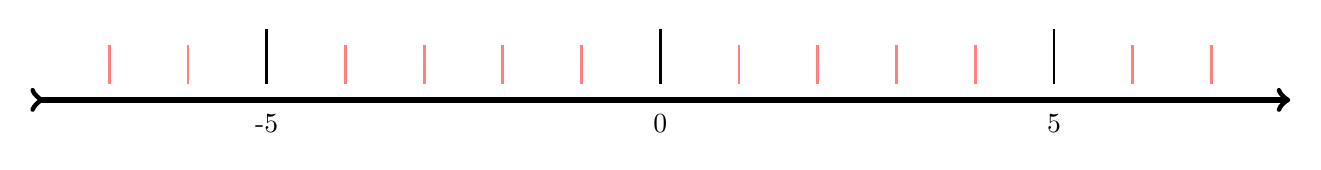
\begin{tikzpicture}
    % Draw the main ruler line from 0 to 2
    \draw[line width=2pt, >->] (-8,0) -- (8,0);
    


    % Draw the larger dashes for 0, 1, and 2
     \foreach \x in {-7,-6,-4,-3,-2,-1,1,2,3,4,6,7}
         \draw[line width=1pt, color=red!50] (\x, 0.2) -- (\x, 0.7);


    % % Draw the smaller dashes for 0.1 to 0.9
     \foreach \x in {-5,0,5}
         \draw[line width=1pt] (\x, 0.2) -- (\x, 0.9) node[below] at (\x,-0.05) {\x};

    % \draw[line width=0.2pt,<-] (3.162,-0.1) -- (3.162,-3) node[below] {$A$};
    % \draw[line width=0.2pt,<-] (0.5,.12) -- (0.5,.2) node[above] {\tiny$B$};
    % \draw[line width=0.2pt,<-] (1.2,.12) -- (1.2,.2) node[above] {\tiny$C$};
    % \draw[line width=0.2pt,<-] (1.6,.12) -- (1.6,.2) node[above] {\tiny$D$};
\end{tikzpicture}
\end{document}